% =====================================================================
%  Fig. 4 -- Auxiliary Convolutional Branch and Weighted Ensemble Head
% =====================================================================
\documentclass[tikz,border=3pt]{standalone}
\usepackage{helvet}
\renewcommand{\familydefault}{\sfdefault}
\usepackage{amsmath,amssymb}
\usetikzlibrary{arrows.meta,positioning,calc,fit,backgrounds,decorations.pathreplacing}

\hyphenpenalty=10000 \exhyphenpenalty=10000 \pretolerance=10000 \tolerance=9999

\definecolor{cGraph}{HTML}{5B4B8A}  \definecolor{cGraphBg}{HTML}{ECE8F6}
\definecolor{cAux}{HTML}{BF7326}    \definecolor{cAuxBg}{HTML}{FBEEDA}
\definecolor{cFuse}{HTML}{9E2A2B}   \definecolor{cFuseBg}{HTML}{F8E5E5}
\definecolor{cTrain}{HTML}{2A9D8F}  \definecolor{cTrainBg}{HTML}{DEF2EF}
\definecolor{cInk}{HTML}{1F2933}

\begin{document}
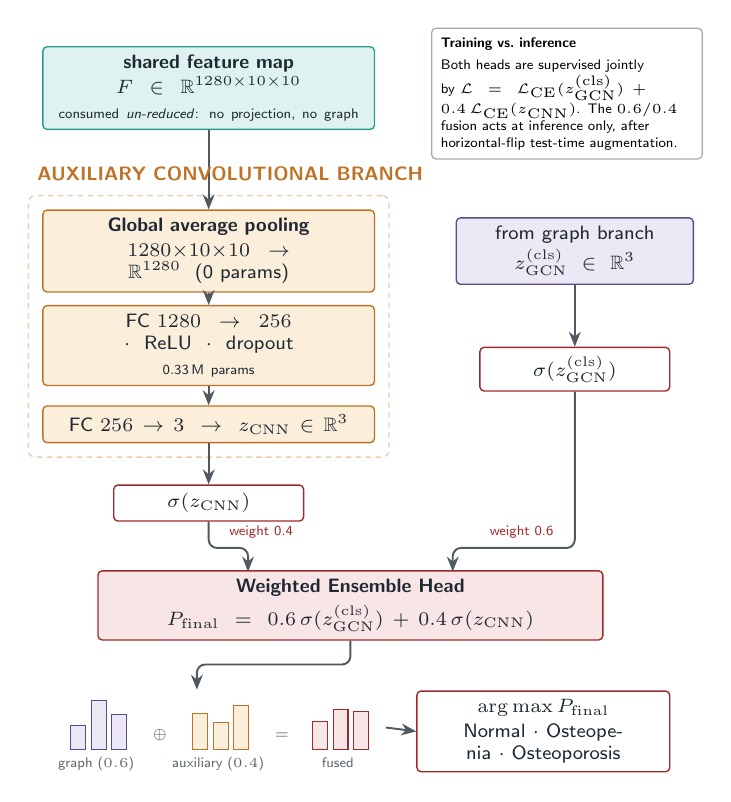
\begin{tikzpicture}[
  font=\scriptsize,
  blk/.style 2 args={draw=#1, fill=#2, rounded corners=1.5pt, line width=.5pt,
                     align=center, text=cInk, inner sep=3pt},
  flow/.style={-{Stealth[length=1.9mm,width=1.5mm]}, line width=.7pt, draw=cInk!78},
  route/.style={-{Stealth[length=1.9mm,width=1.5mm]}, line width=.7pt, draw=cInk!78,
                rounded corners=3pt},
  shp/.style={font=\tiny, text=cInk!72, inner sep=1pt},
  ttl/.style={font=\scriptsize\bfseries, text=#1},
  panel/.style={draw=#1!35, rounded corners=2.5pt, line width=.5pt,
                dash pattern=on 2pt off 1.6pt},
]

% ---------------- shared feature map ----------------
\node[blk={cTrain}{cTrainBg}, text width=40mm] (F) at (2.30,9.62)
  {\textbf{shared feature map}\\[1pt] $F\in\mathbb{R}^{1280\times10\times10}$\\[1pt]
   {\tiny consumed \emph{un-reduced}: no projection, no graph}};

% ---------------- auxiliary branch ----------------
\node[blk={cAux}{cAuxBg}, text width=40mm] (gap) at (2.30,7.55)
  {\textbf{Global average pooling}\\[1pt]
   $1280{\times}10{\times}10 \rightarrow \mathbb{R}^{1280}$\ \ (0 params)};
\node[blk={cAux}{cAuxBg}, text width=40mm] (fc1) at (2.30,6.35)
  {FC $1280 \rightarrow 256$\ \ $\cdot$\ \ ReLU\ \ $\cdot$\ \ dropout\\[1pt]
   {\tiny 0.33\,M params}};
\node[blk={cAux}{cAuxBg}, text width=40mm] (fc2) at (2.30,5.35)
  {FC $256 \rightarrow 3\ \rightarrow\ z_{\mathrm{CNN}}\in\mathbb{R}^{3}$};

\draw[flow] (F) -- (gap);
\draw[flow] (gap) -- (fc1);
\draw[flow] (fc1) -- (fc2);

\begin{scope}[on background layer]
  \node[panel=cAux, fit=(gap)(fc2), inner sep=5pt] (laneAux) {};
\end{scope}
\node[ttl=cAux, anchor=south west] at ($(laneAux.north west)+(0,0.6mm)$)
  {AUXILIARY CONVOLUTIONAL BRANCH};

% ---------------- incoming graph logits ----------------
\node[blk={cGraph}{cGraphBg}, text width=28mm] (zg) at (6.95,7.55)
  {from graph branch\\[1pt] $z^{(\mathrm{cls})}_{\mathrm{GCN}}\in\mathbb{R}^{3}$};

% ---------------- softmax ----------------
\node[blk={cFuse}{white}, text width=22mm] (sm1) at (6.95,6.05)
  {$\sigma(z^{(\mathrm{cls})}_{\mathrm{GCN}})$};
\node[blk={cFuse}{white}, text width=22mm] (sm2) at (2.30,4.35)
  {$\sigma(z_{\mathrm{CNN}})$};

\draw[flow] (zg) -- (sm1);
\draw[flow] (fc2) -- (sm2);

% ---------------- fusion ----------------
\node[blk={cFuse}{cFuseBg}, text width=62mm] (fuse) at (4.10,3.05)
  {\textbf{Weighted Ensemble Head}\\[2pt]
   $P_{\mathrm{final}} = 0.6\,\sigma(z^{(\mathrm{cls})}_{\mathrm{GCN}})
    + 0.4\,\sigma(z_{\mathrm{CNN}})$};

\draw[route] (sm1.south) -- (6.95,3.78) -- (5.40,3.78) -- (5.40,3.48);
\draw[route] (sm2.south) -- (2.30,3.78) -- (2.80,3.78) -- (2.80,3.48);
\node[shp, text=cFuse, anchor=east] at (6.72,3.98) {weight 0.6};
\node[shp, text=cFuse, anchor=west] at (2.52,3.98) {weight 0.4};

% ---------------- probability illustration ----------------
\draw[route] (fuse.south) -- (4.10,2.30) -- (2.15,2.30) -- (2.15,1.98);

\begin{scope}[shift={(0.55,1.22)}]
  \foreach \i/\h in {0/0.30, 1/0.62, 2/0.44}{
    \draw[draw=cGraph, fill=cGraphBg, line width=.4pt]
      (\i*0.26,0) rectangle ++(0.19,\h);}
  \node[shp, anchor=north] at (0.32,-0.06) {graph ($0.6$)};
\end{scope}
\node[shp] at (1.68,1.40) {$\oplus$};
\begin{scope}[shift={(2.10,1.22)}]
  \foreach \i/\h in {0/0.46, 1/0.34, 2/0.56}{
    \draw[draw=cAux, fill=cAuxBg, line width=.4pt]
      (\i*0.26,0) rectangle ++(0.19,\h);}
  \node[shp, anchor=north] at (0.32,-0.06) {auxiliary ($0.4$)};
\end{scope}
\node[shp] at (3.23,1.40) {$=$};
\begin{scope}[shift={(3.62,1.22)}]
  \foreach \i/\h in {0/0.36, 1/0.51, 2/0.48}{
    \draw[draw=cFuse, fill=cFuseBg, line width=.4pt]
      (\i*0.26,0) rectangle ++(0.19,\h);}
  \node[shp, anchor=north] at (0.32,-0.06) {fused};
\end{scope}

\node[blk={cFuse}{white}, text width=30mm] (pred) at (6.55,1.45)
  {$\arg\max P_{\mathrm{final}}$\\[1pt]
   Normal $\cdot$ Osteopenia $\cdot$ Osteoporosis};
\draw[flow] (4.55,1.50) -- (pred.west);

% ---------------- side note ----------------
\node[draw=cInk!40, fill=white, rounded corners=1.5pt, line width=.45pt,
      align=left, text width=32mm, font=\tiny] (note) at (6.85,9.55)
  {\textbf{Training vs.\ inference}\\[2pt]
   Both heads are supervised jointly by
   $\mathcal{L}=\mathcal{L}_{\mathrm{CE}}(z^{(\mathrm{cls})}_{\mathrm{GCN}})
    +0.4\,\mathcal{L}_{\mathrm{CE}}(z_{\mathrm{CNN}})$.
   The $0.6/0.4$ fusion acts at inference only, after horizontal-flip
   test-time augmentation.};

\end{tikzpicture}
\end{document}
